\chapter{Le forzanti del sistema climatico}
\section{Introduzione}
Il clima è lo stato e l’insieme statistico di un sistema climatico, che possiamo definire in tanti modi con tanti livelli di difficoltà. Riscostruzione delle seie temporali partendo da uno sguardo che ci danno i nostri proxies. Modelli che usano circa 10km di lato di quadrato nella modellizzazione. “Climate is the composite or generalization of weather conditions of a region”. 

Forzante esterna: una serie di effetti che interferiscono alla variabilità “variabilità forzata” attribuita ad un agente esterno responsabile. Oceano ha tempi caratteristici molto più lunghi che possono permetterci di spiegare alcune fluttuazioni. 

Variabilità interannuale in cui emergono tanti processi con conseguenze immediate sul clima superficiale (ENSO). Global circulation è fondamentale per spiegare questo tipo di comportamento di distribuzione delle temperature. Alternanza terra-mare, presenza di ghiaccio, orografia contribuiscono alla distribuzione longitudinale della temperatura. 

Nel caso delle precipitazioni serve studiare qualcosa in più: il trasporto di energia o masse d’aria per comprendere la distribuzione delle precipitazioni.

Nel mediterraneo esistono zone di storm track minori, ma guardano al generale vi sono tracks du cicloni extratropicali. 

La statistica di una variabile meterologica in questi dati devo simulare dei processi molto veloci. 

Rwmwmbwer: atmosfera è un fluido forzato, dissipativo, stratificato in un sistema rotante. Lo studio del clima non può prescindere da quello che viene su scale temporali molto brevi.

NAO. Processo di Low frequency variability.

\begin{figure}[htpb]
    \centering
    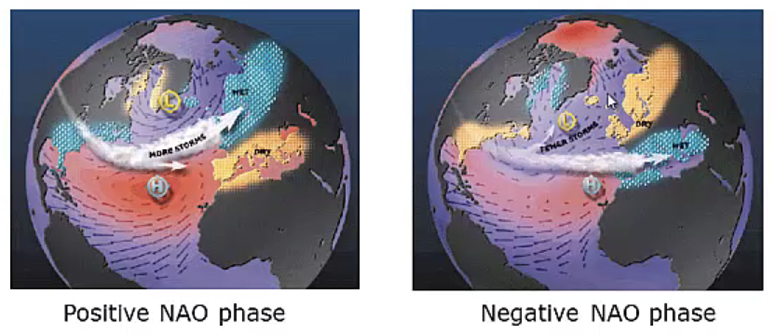
\includegraphics[width=0.5\linewidth]{uploads/NAO phases.png}
\end{figure}
Blocking atmpspheric: processo di ostacolo che ferma la corrente, altro processo di low freq stability in tempi più lunghi della low freq variability c’è ad esempio El Nino Southern Oscillation: pulsazione della fascia equatoriale del pacifico. Delle piccole perturbazioni distruggono l’equilibro facendoci entrare in uno stato di disturbazione El Nino. Statistica stagionale nella variailità 

Come prima queste fluttuazioni di t sono spiegate da simmetrie orografiche. 

El nino teleconnections: introduzione di (a)simmetrie che si ripercuotono nella statistica 


\section{Variabilità multidecadiale}
In una scala temporale in cui si mischiano molto le variabiliti naturali con le forzanti esterne. Atlantic multi-decadial variability caratterizzata da pulsazione di tempi molto lunghi con comportamento quasi periodico di 6 decenni. Principale motore della previsione decadale. Punto di confine tra i tempi su chui è importante considerare la var nat e tempi in cui (più di 10 anni) in cui se considero la temperatura di 50 anni davanti a me non mi aspetto di vedere un ruolo significativo di fenomeni natural ma forzanti climatiche antropogeniche. 

Se osservassi la temperatura da un satellite coe sarebbe la temperatura di emissione della Terra? 255K. Perché è diversa dalla temperatura che osserviamo sulla superficie? Per l’effetto serra.







Che significato ha questa $T$? La temperatura di emissione $T_e$ è un buon modello della temperatura superficiale della Terra? Come interpretarlo e come determinare se è un buon modello? Questa $T_e$ è la temperatura che stimiamo dallo spazio, ma non è puramente rappresentativa della temperatura superficiale.
L'effetto serra naturale in un pianeta è semplificato nel fatto che lascia passare la radiazione solare ma non la radiazione terrestre.
Ci sono dei tipi di radiazione (lunghezza d'onda centrale) che rendono l'atmosfera opaca. 
L'atm influisce sulla temperatura terrestre tramite effetto serra, lo fa per effetto di alcune molecole presenti: cambiando la composizione chimica cambia effetto. 
$T_s$ è mantenuta più alta dal fluido atmosferico che trattiene l'energia emessa dalla superficie terrestre non trasformandola in energia out.



Gas serra rendono una parte dell'atmosfera sostanzialmete opaca senza andare ad alterare l'assorbimento della radiazione solare.
\begin{figure}[htpb]
    \centering
    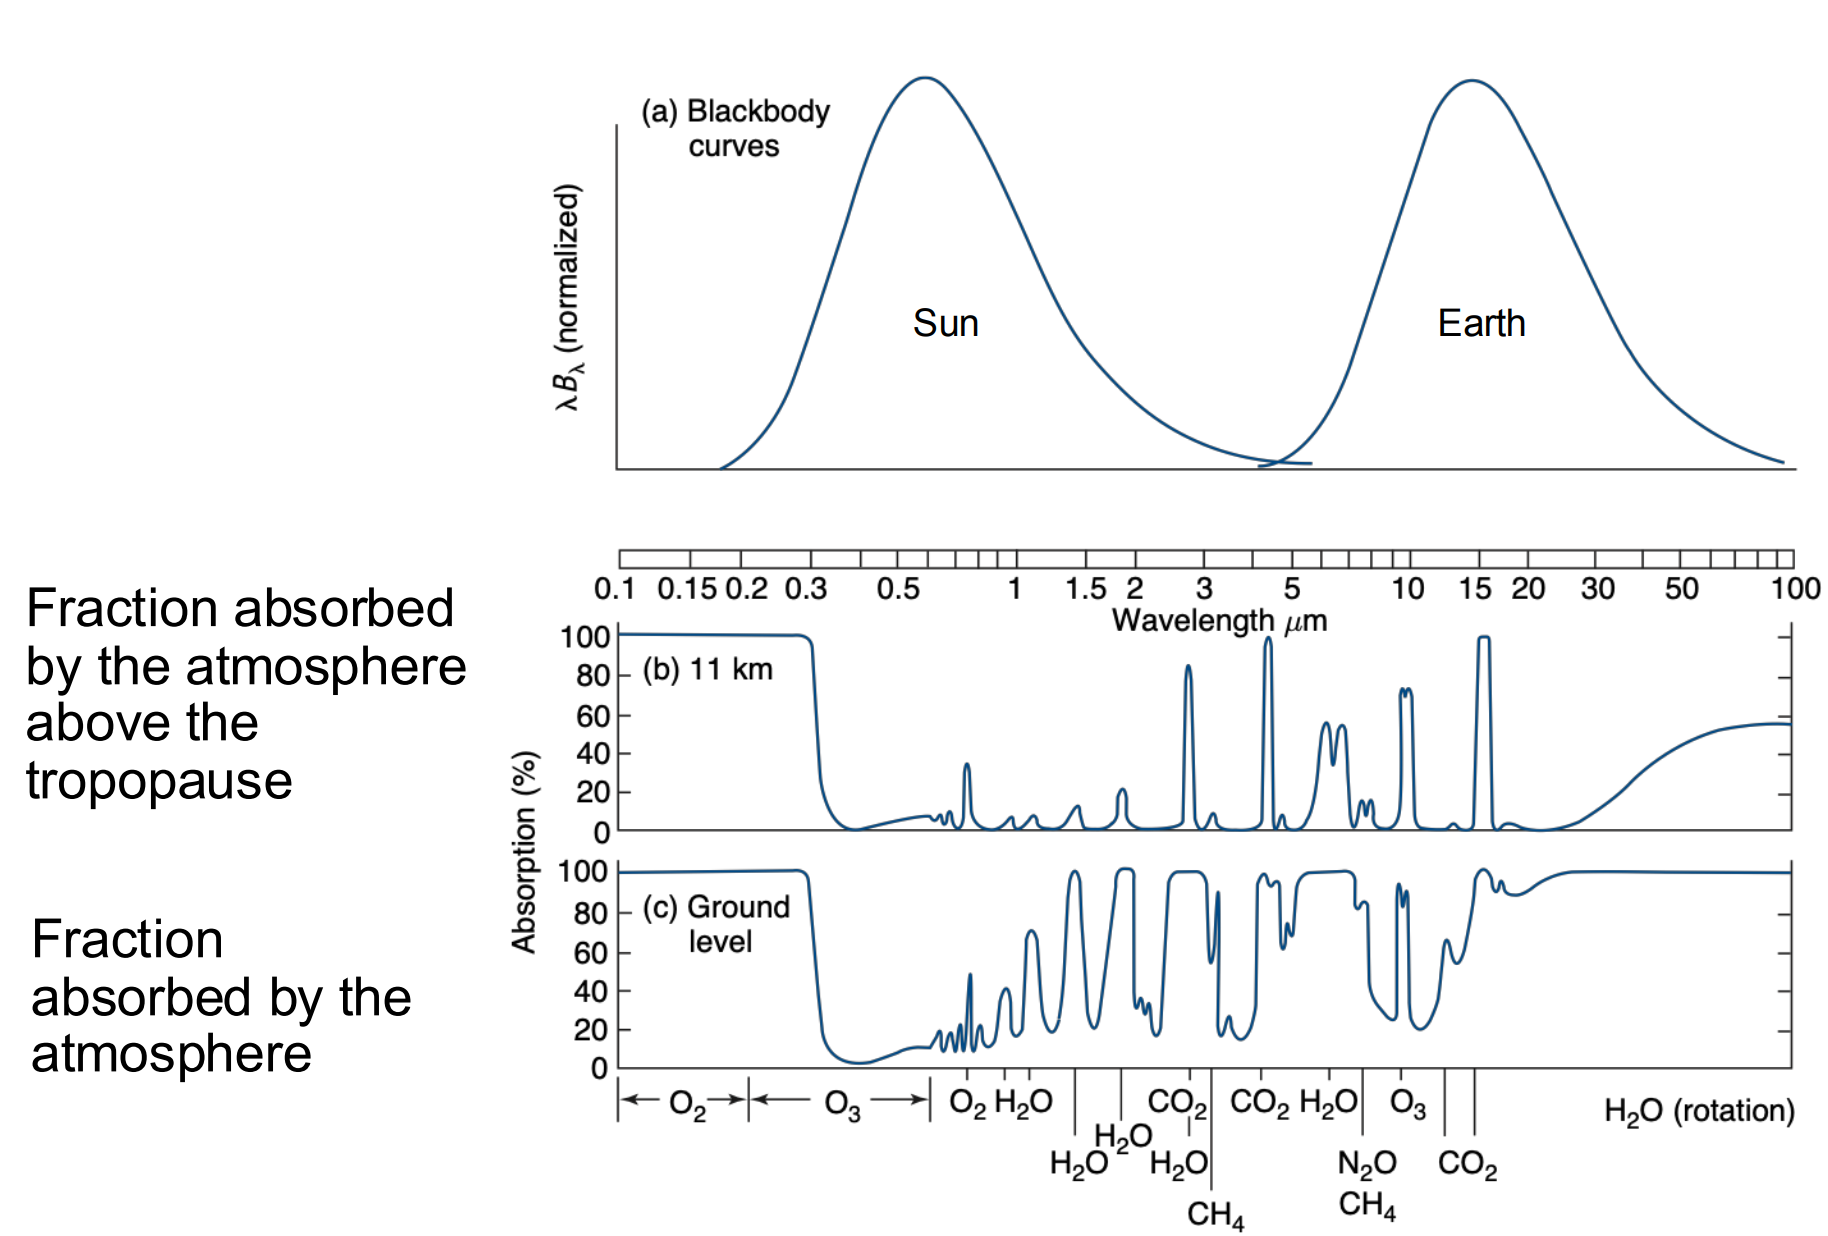
\includegraphics[width=0.5\linewidth]{uploads/ass terr.png}
    \label{fig:fin atm}
\end{figure}
\paragraph{Modelli per il GH effect}
è la riemissione dell'atmosfera che scalda la superficie terrestre. Da fuori vedo la temperatura dell'atmosfera $T_e=T_a$. Solar input non interagisce con l'atmosfera, nell'input solare c'è da considerare l'albedo obv. In realtà c'è una parte che scappa $\varepsilon$ (nella figura \ref{fig:fin atm} a grandi wavelength) che rappresenta la trasmissività che regola quanta radiazione rimane nella superficie: quanto ho popolato l'atm con gas che sono in grado di interagire. Forzante radiativa: quanto cambia la temperatura per un aumento della co2.
\begin{figure}[htpb]
    \centering
    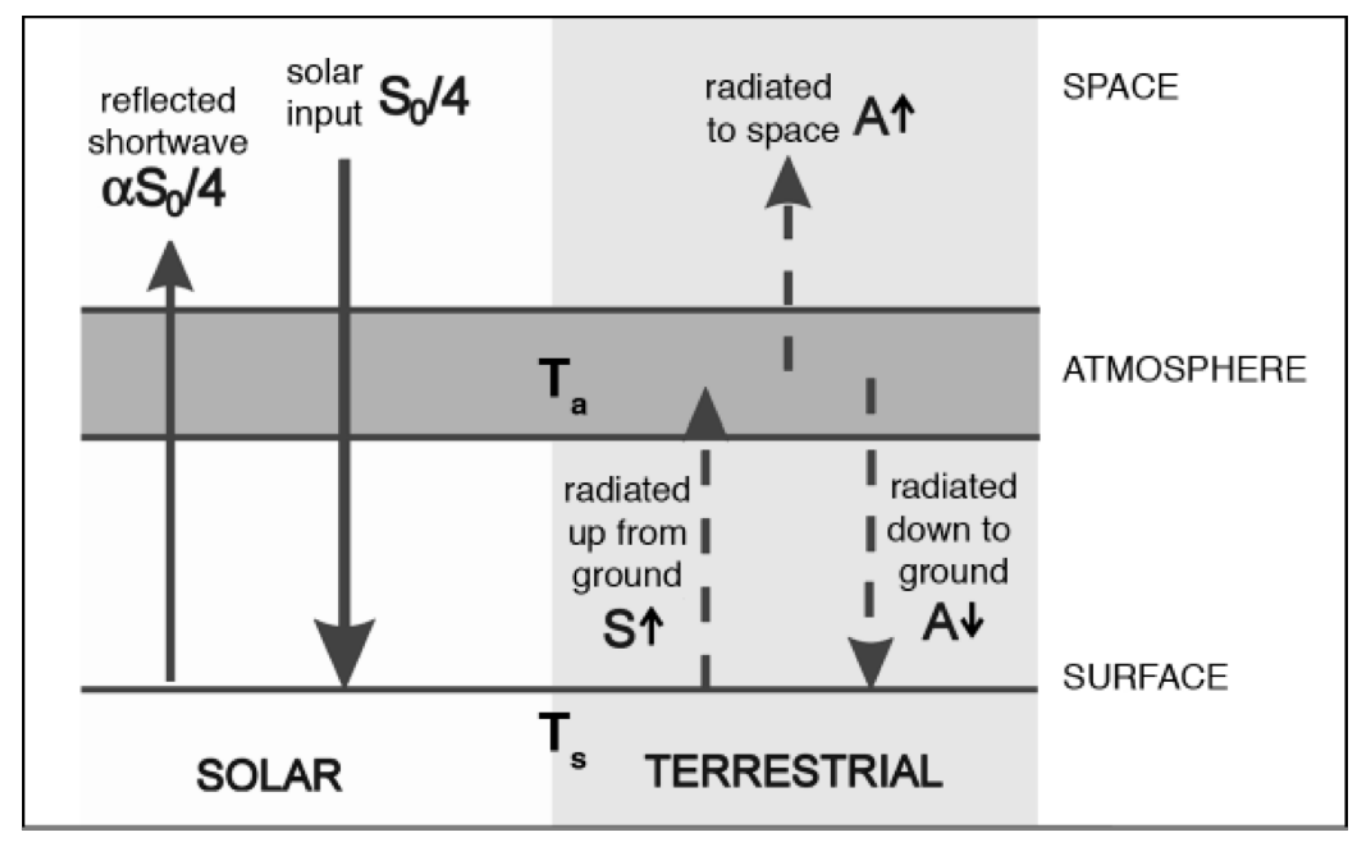
\includegraphics[width=0.5\linewidth]{uploads/GH effect.png}
\end{figure}
\section{Climate sensitivity}
\paragraph{The Charney report} The science of Joule Charney ed Lorentz, è il primo assessment scientifico intorno al tema di carbon dioxide e clima.

Problema transiente: come il clima risponderà per variazioni negli anni futuri. \textit{Trustworthy and actionable}.
\begin{center}
    "The primary effect of an increase of CO$_2$ is to cause more absorption of thermal radiation from the earth's surface and thus to increase the air temperature in the troposphere"
\end{center}
Quanto $T_S>T_e$ dipende dalla capacità dell'atm di trattenere l'energia: $T_s(\varepsilon)$ superficiale. L'atm vede l'introduzione di gas come una perturbazione molto grande anche se piccola dal punto di vista di ciclo biochimico. Il risultato della loro analisi è un $\Delta T\simeq 3\pm 1..5$°C. per un raddoppio di CO$_2$. 
GCM cercano di rappresentare tutta la complessità, questi invece partono da posizioni più "semplici" di controllo che sono controllabili più facilmente; questi due approcci nell'assessment danno \textit{similar results}. 
\paragraph{The 4th IPCC report} \begin{center}
    "Warming oof the climate system is unequivocal, as is now evident from observations of increases in global average air and ocean temperatures, widespread melting of snow and ice, and rising global average sea level"
\end{center}
\subsection{Global radiative balance}
\begin{figure}[htpb]
    \centering
    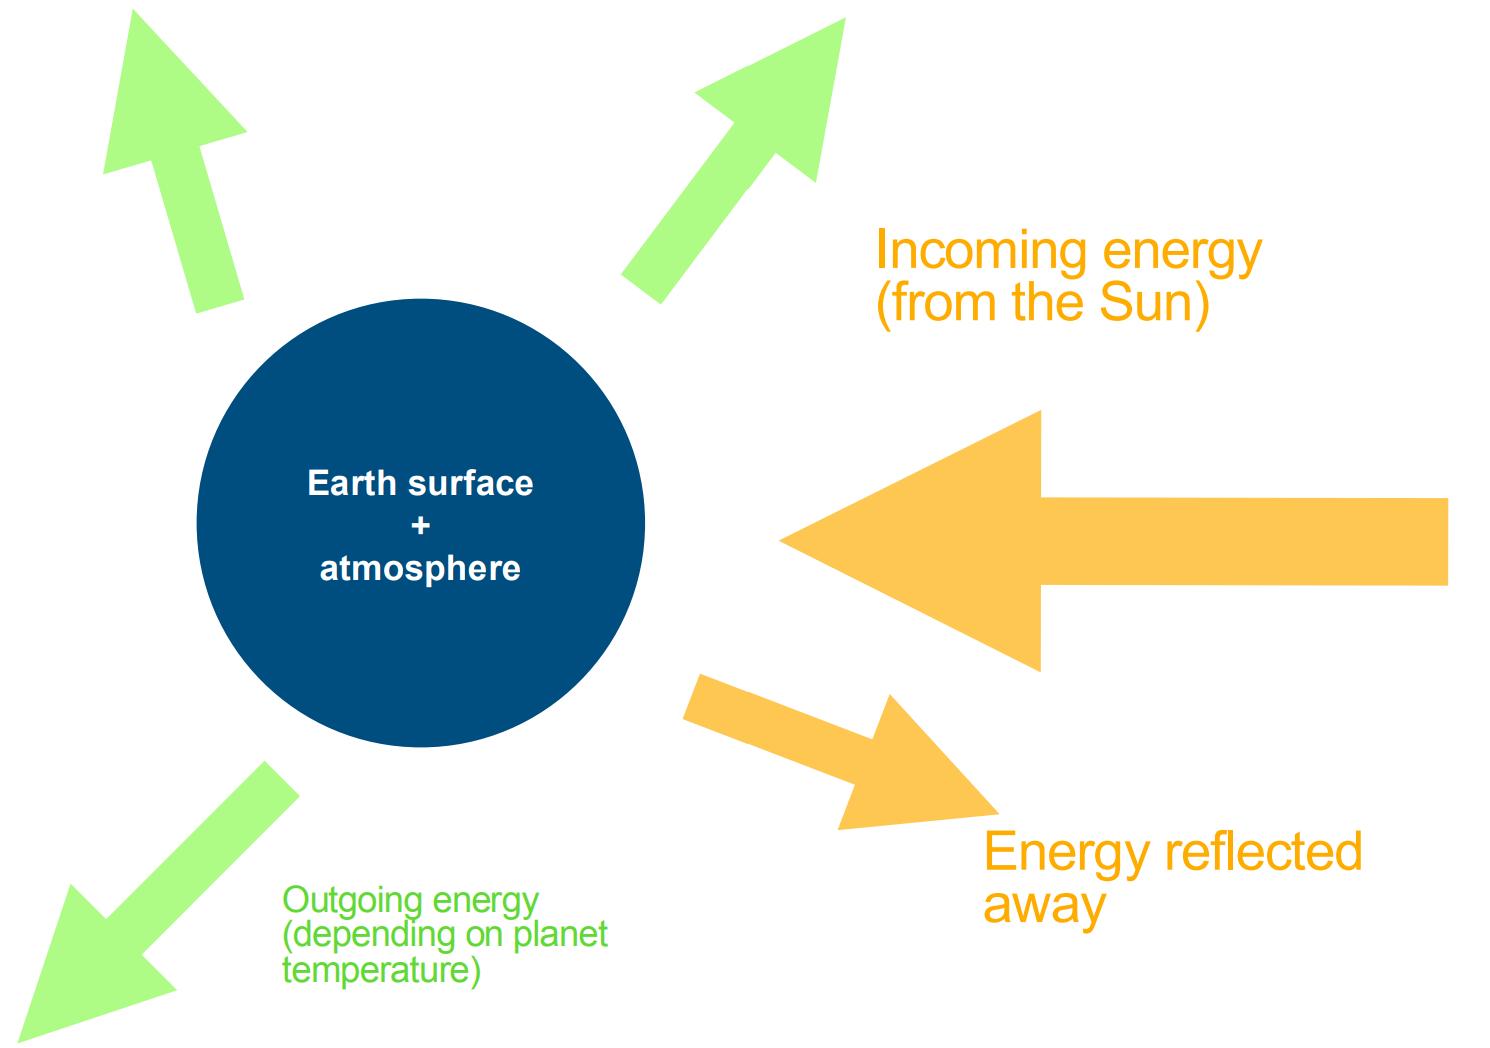
\includegraphics[width=0.5\linewidth]{uploads/GRB.png}
    \caption{Global radiative balance tra energia che entra ed esce}
\end{figure}
Che succede se trattengo un po' di questa energia intorno alla Terra e vedo cosa succede nel sistema. La prima importante risposta del sistema è emettere più energia=scaldarsi. Quanto si deve scaldare il pianeta per il ristabilirsi di un nuovo equilibrio? (Domanda che si sono fatti nel report)
Balanced eq:
$$\frac{Q_0}{4}(1-\alpha)-\sigma T^4=0$$
ma poi supponiamo un imbalance:
$$\frac{Q_0}{4}(1-\alpha)+\Delta R-\sigma T^4\neq0$$
Allora stiamo cercando una nuova temperatura che emetto per stare di nuovo in eq posto che un po' ne sto trannenendo con $\Delta R$, $T_{\text{new}}$ cosicché:
\begin{equation}
    \frac{Q_0}{4}(1-\alpha)+\Delta R-\sigma (T_{\text{new}})^4=0
\end{equation}
con $$T_{\text{new}}=T+\Delta T$$
approximating:
$$(T+\Delta T)^4\approx T^4+4T^3\Delta T$$
Hence, 
\begin{equation}
\begin{split}
     & \frac{Q_0}{4}(1-\alpha)+\Delta R-\sigma ( T^4+4T^3\Delta T)=0\\
     & \Leftrightarrow \cancel{\frac{Q_0}{4}(1-\alpha)}+\Delta R\cancel{-\sigma  T^4}+4\sigma T^3\Delta T=0\\
     &\Leftrightarrow \Delta R=4\sigma T^3\Delta T
\end{split}
\end{equation}
Posso fare quindi una proporzione tra delta climate and delta radiative forcing: 
$$\Delta T=\lambda\Delta R$$
dove $T$ è la temperatura dell'equilibrio iniziale. Perturbo eq, raggiungo un nuovo eq che è ottenuto scaldando il pianeta in modo da bilanciare la forzante radiativa. Come faccio? Devo ottenere una stima di $\lambda$ che tenga conto anche di altri pezzi, non solo la temperatura. Ma il primo metodo di stima è questo, tutto il lavoro dopo è migliorare la stima di $\lambda$: coefficiente che dice quanto cambia $T$ del pianeta in risposta a una forzante radiativa. $$\lambda\approx 0.25 \text{ K/(W/m}^2)$$
Poi potrei contare tutti i feedback che influiscono sulla forzante. Considerando nuovi feedback, $\lambda$ era tale da essere circa $3$ K/(W/m$^2$). Alcuni di questi feedback sono il sea-ice, GHGs. 
\begin{figure}[htpb]
    \centering
    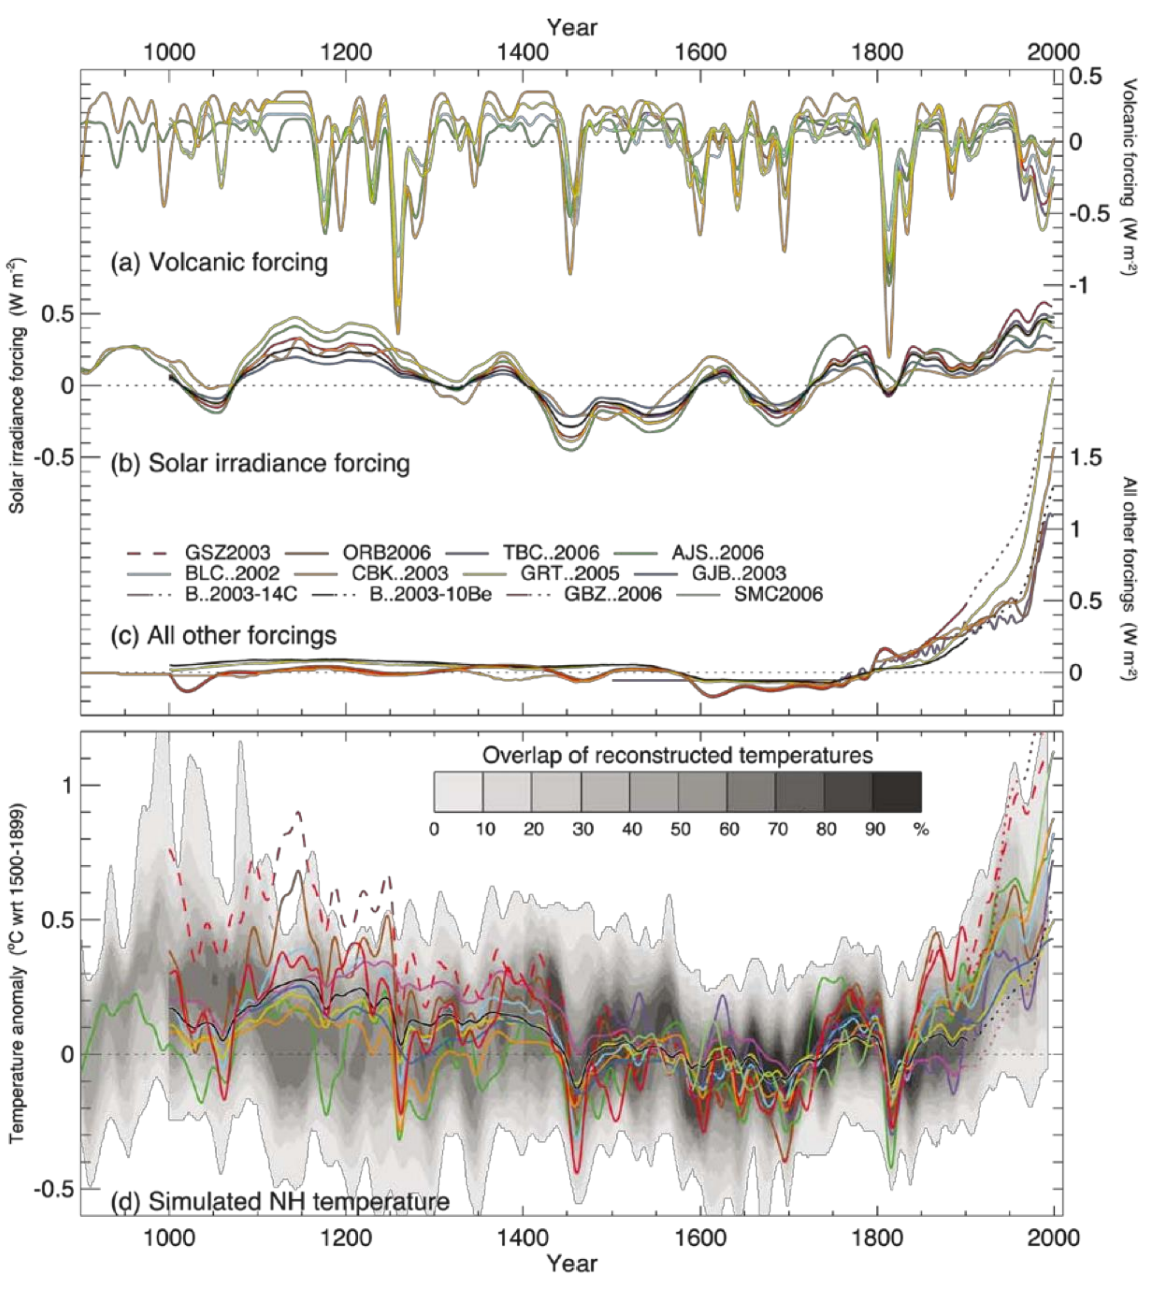
\includegraphics[width=0.5\linewidth]{uploads/Climate.png}
    \caption{We have been able to simulate the climate of the past with natural radiative forcing.}
\end{figure}
\begin{figure}[htpb]
    \centering
    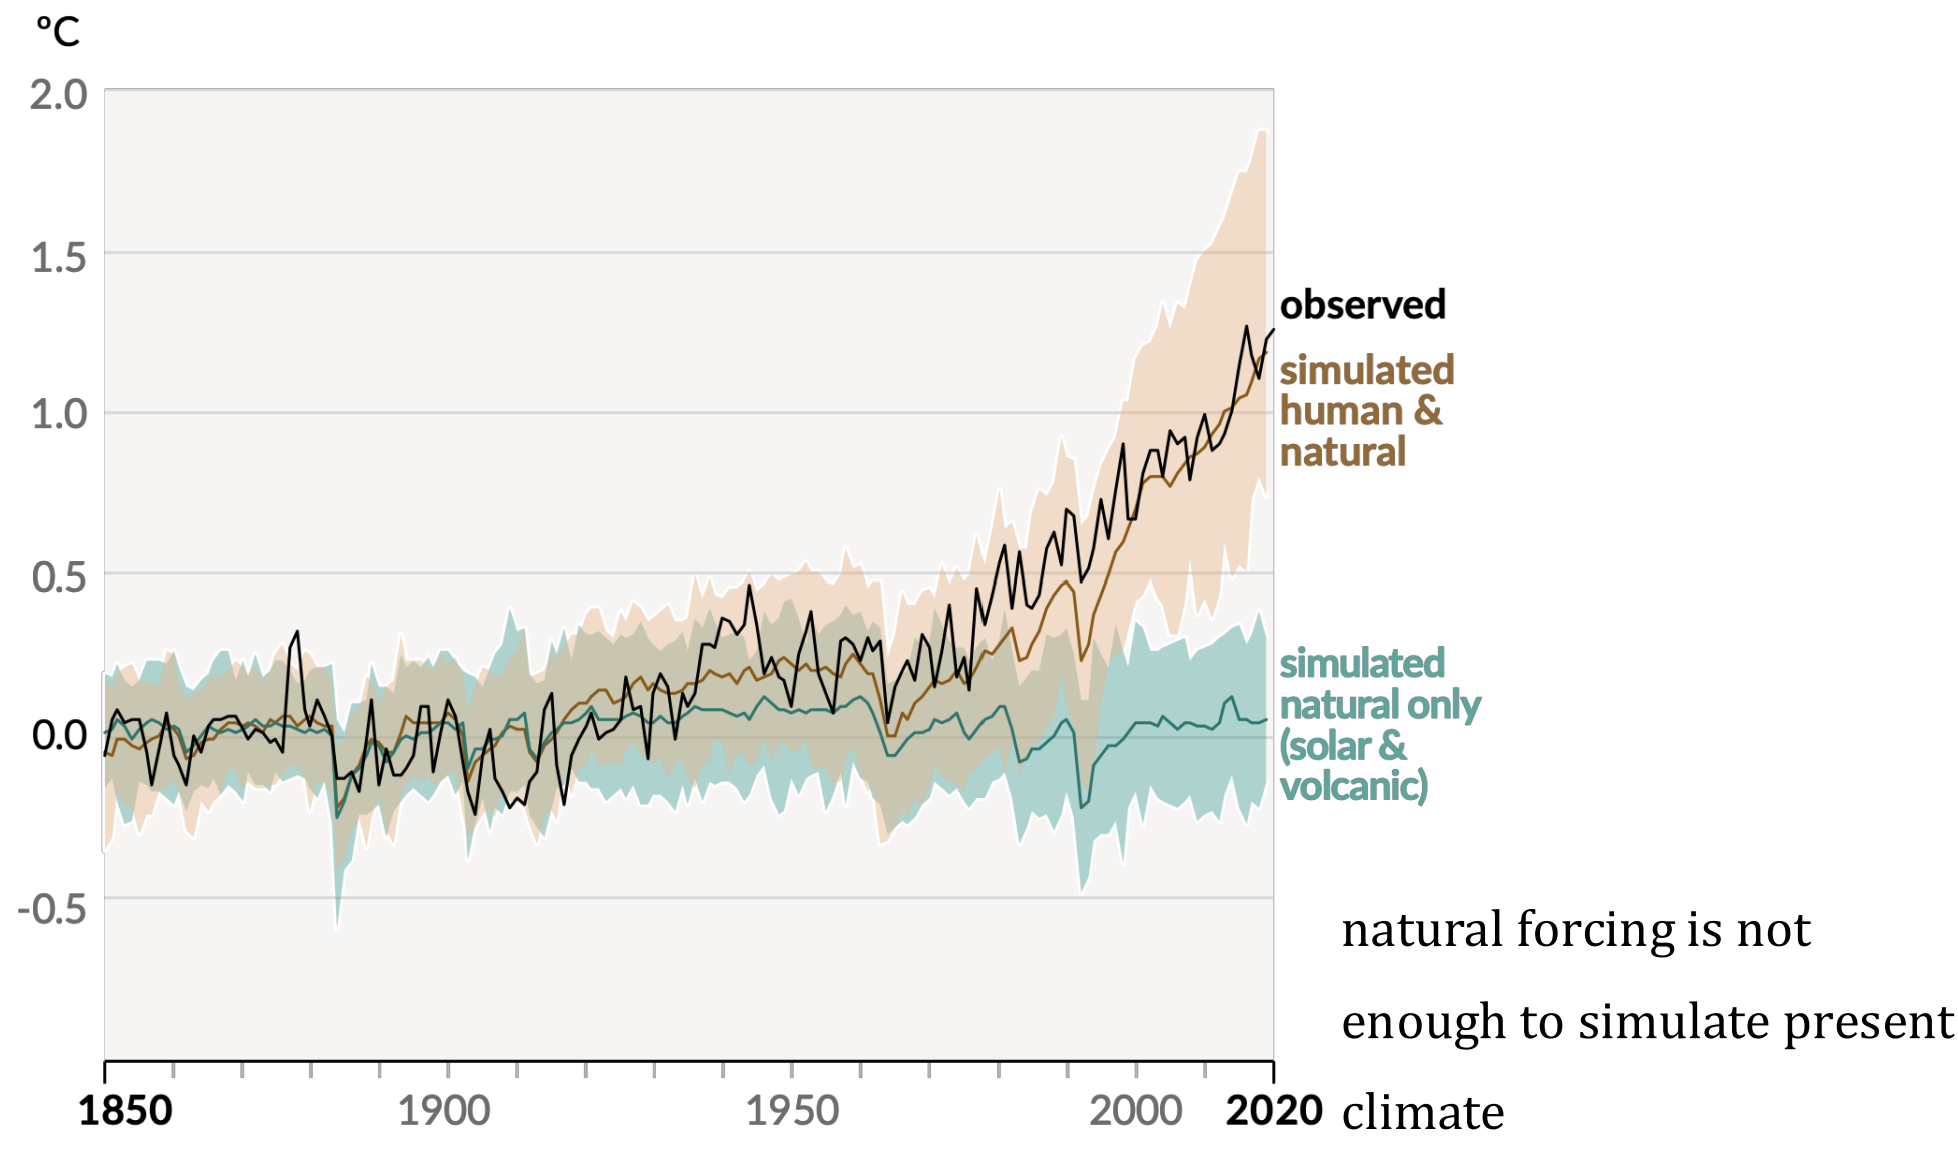
\includegraphics[width=0.5\linewidth]{uploads/models.png}
\end{figure}
C'è evidenza nella osservazione, non c'è dubbio scettico ora.

Il futuro della previsione climatica è il cambiamento climatico regionale actionable. Il passo in avanti è che ora abbiamo capito come stimare il cambiamento climatico regionale.
Approcci semplici e complessi che possono dare pov interessanti a modo loro.


Facile la policy sull'adattamento, è bottom up (parte dal locale) (UE l'ha fatto) ma mitigation (è top down: serve coordinamento a livello internazionale)?

La community scientifica non dà probabilità a questi scenari, ma analizza semplicemente la risposta agli diversi stimoli. Check out technical summary of IPCC.